% Universidad Nacional de Loja | Programación Web
% Cristhian Hipólito Girón Chamba | Docente: Johnny H. Sánchez L.
% Bitácora documental del SGP. Edición: 10 de noviembre de 2026.
% Compilar dos veces con pdfLaTeX desde esta carpeta; conservar imagenes/.
% No requiere PlantUML ni shell-escape.
\documentclass[11pt,a4paper]{article}
\usepackage[utf8]{inputenc}
\usepackage[T1]{fontenc}
\usepackage{lmodern}
% Usa español cuando está instalado; conserva la compilación en TeX Live básico.
\IfFileExists{spanish.ldf}{\usepackage[spanish,es-tabla]{babel}}{}
\usepackage[margin=2.4cm,headheight=15pt]{geometry}
\usepackage{xcolor,graphicx,array,longtable,booktabs,fancyhdr,microtype,listings}
\graphicspath{{imagenes/}}
\usepackage[unicode,colorlinks=true,linkcolor=azul,urlcolor=azul]{hyperref}
\definecolor{azul}{HTML}{173B59}
\definecolor{oro}{HTML}{B39759}
\definecolor{gris}{HTML}{52616B}
\definecolor{suave}{HTML}{F2F5F7}

\definecolor{codigoverde}{HTML}{276454}
\lstdefinestyle{sgpjava}{
 language=Java,basicstyle=\ttfamily\footnotesize,
 keywordstyle=\color{azul}\bfseries,stringstyle=\color{codigoverde},
 commentstyle=\color{gris},backgroundcolor=\color{suave},
 frame=l,rulecolor=\color{oro},framerule=1pt,
 numbers=left,numberstyle=\tiny\color{gris},numbersep=8pt,
 xleftmargin=18pt,framexleftmargin=6pt,framesep=6pt,
 breaklines=true,breakatwhitespace=false,columns=fullflexible,
 keepspaces=true,showstringspaces=false,tabsize=4,
 aboveskip=8pt,belowskip=8pt,
 literate={á}{{\'a}}1 {é}{{\'e}}1 {í}{{\'i}}1 {ó}{{\'o}}1 {ú}{{\'u}}1
          {ñ}{{\~n}}1 {Á}{{\'A}}1 {É}{{\'E}}1 {Í}{{\'I}}1 {Ó}{{\'O}}1 {Ú}{{\'U}}1
}

\hypersetup{pdftitle={Bitácora del proyecto SGP},pdfauthor={Cristhian Hipólito Girón Chamba},pdfsubject={Registro documental, interfaces y secuencias principales}}
\renewcommand{\contentsname}{Índice}
\renewcommand{\tablename}{Tabla}
\renewcommand{\figurename}{Figura}
\setlength{\parindent}{0pt}
\setlength{\parskip}{6pt}
\setlength{\emergencystretch}{2em}
\renewcommand{\arraystretch}{1.2}
\setlength{\tabcolsep}{5pt}
\pagestyle{fancy}
\fancyhf{}
\fancyhead[L]{\small\color{azul}SGP\enspace /\enspace Bitácora del proyecto}
\fancyhead[R]{\small\color{gris}Programación Web}
\fancyfoot[L]{\small\color{gris}Universidad Nacional de Loja}
\fancyfoot[R]{\small\thepage}
\renewcommand{\headrulewidth}{0.4pt}
\newcolumntype{P}[1]{>{\raggedright\arraybackslash}p{#1}}
\newcommand{\ruta}[1]{{\small\path{#1}}}
\newcommand{\nota}[1]{\par\smallskip\begingroup\setlength{\fboxsep}{9pt}\colorbox{suave}{\parbox{\dimexpr\linewidth-18pt\relax}{\small #1}}\endgroup\par\smallskip}
% Diagramas vectoriales nativos de LaTeX. Coordenadas en milímetros.
\newcommand{\msg}[5]{\put(#1,-#3){\vector(#4,0){#2}}\put(#1,-#3){\makebox(0,0)[bl]{\raisebox{2mm}{\colorbox{white}{\scriptsize #5}}}}}
\newcommand{\ret}[5]{\put(#1,-#3){\vector(#4,0){#2}}\put(#1,-#3){\put(-#2,0){\makebox(0,0)[bl]{\raisebox{2mm}{\colorbox{white}{\scriptsize #5}}}}}}
\newcommand{\local}[3]{\put(#1,-#2){\line(1,0){5}\put(5,0){\line(0,-1){2}}\put(5,-2){\vector(-1,0){5}}}\put(#1,-#2){\makebox(0,0)[bl]{\raisebox{2mm}{\colorbox{white}{\scriptsize #3}}}}}
\begin{document}
\begin{titlepage}
\thispagestyle{empty}
\begin{center}

\includegraphics[width=6.4cm]{unl-logo.png}\par
\vspace{2mm}
{\large\bfseries\color{azul} UNIVERSIDAD NACIONAL DE LOJA\par}
\vspace{3mm}
{\normalsize Pedagogía de las Ciencias Experimentales\par}
{\normalsize Informática\par}
\vspace{3mm}
{\small\color{gris} PROGRAMACIÓN WEB\par}
\end{center}
\vspace{7mm}
{\color{oro}\rule{\linewidth}{1pt}\par}
\vspace{7mm}
\begingroup
\setlength{\fboxsep}{18pt}
\noindent\colorbox{azul}{\parbox{\dimexpr\linewidth-36pt\relax}{%
\color{white}
{\small DOCUMENTACIÓN DEL PROYECTO\par}
\vspace{6mm}
{\fontsize{33}{37}\selectfont\bfseries Bitácora\par del proyecto\par}
\vspace{6mm}
{\Large Sistema de Gestión de Prácticas\par}
\vspace{2mm}
{\large\color{oro} SGP\par}
}}
\endgroup\par
\vspace{6mm}
{\color{gris} Análisis y evolución del sistema\par}
{\small\color{gris} Requisitos, interfaces, secuencias y algoritmos relevantes\par}
\vfill
{\small\bfseries\color{azul} DATOS ACADÉMICOS\par}
\vspace{2mm}
\begingroup
\setlength{\fboxsep}{12pt}
\noindent\colorbox{suave}{\parbox{\dimexpr\linewidth-24pt\relax}{%
\begin{tabular}{@{}P{2.3cm}P{11.2cm}@{}}
\textbf{Autor} & Cristhian Hipólito Girón Chamba\\
\textbf{Correo} & \href{mailto:cristhian.giron@unl.edu.ec}{cristhian.giron@unl.edu.ec}\\
\textbf{Docente} & Johnny H. Sánchez L.\\
\textbf{Asignatura} & Programación Web\\
\end{tabular}
}}
\endgroup\par
\vspace{8mm}
{\color{oro}\rule{\linewidth}{0.6pt}\par}
{\small\color{gris} Loja, Ecuador\hfill Edición 1.2\par}
{\small\color{gris} 10 de noviembre de 2026\par}
\end{titlepage}
\pagenumbering{roman}
\tableofcontents
\clearpage
\pagenumbering{arabic}
\section{Presentación y alcance}
En esta bitácora documento el desarrollo del Sistema de Gestión de Prácticas
(SGP), desde la definición de actores y requisitos hasta la implementación de
sus flujos principales. Presento la estructura del proyecto, las interfaces,
los diagramas de casos de uso y secuencia, y los algoritmos que sustentan las
reglas de revisión, asistencia y guardado de borradores.

\textbf{Propósito del proyecto.} Centralizar la gestión de prácticas académicas:
asignación de estudiantes y tutores, elaboración y revisión de documentos,
evidencias, jornadas, asistencias y seguimiento, con acceso según rol y ámbito.

\textbf{Objetivo de la bitácora.} Registrar las actividades realizadas, las
decisiones técnicas, los resultados de las verificaciones y los aspectos
pendientes del proyecto.

\nota{Los resultados de las verificaciones corresponden a las fechas y entornos
indicados en cada informe. Las pruebas con datos simulados, la integración H2 y
las comprobaciones de la instalación local tienen alcances diferentes.}

\subsection{Organización de las fuentes}
La especificación \ruta{docs/requisitos/especificacion.md} es el catálogo principal.
Los informes de \ruta{docs/testing/informes/} registran revisiones fechadas.
La guía \ruta{docs/requisitos/secuencia-login.md} explica la abstracción del login,
y \ruta{docs/requisitos/artefactos/diagrama-secuencia-login.puml} conserva su fuente.
Los documentos de producto, API y desarrollo amplían el contexto técnico.

\subsection{Diferencias entre el catálogo y las últimas decisiones}
El informe del 9 de noviembre sobre asignación administrativa registra que el
estudiante recibe una práctica aprobada y que se eliminaron sus rutas de solicitud
y cancelación. También establece una pertenencia académica activa por estudiante
y ciclo, permitiendo pertenencias en ciclos distintos de su carrera.

El catálogo aún contiene referencias al flujo anterior de solicitud estudiantil.
Se transcribe íntegro en esta edición como \textbf{registro documental}, sin
presentar esas filas como política operativa vigente. Para la decisión más reciente
se consulta \ruta{docs/testing/informes/2026-11-09/asignacion-administrativa-practicas.md}.

El diagrama general \ruta{docs/requisitos/artefactos/diagrama-casos-de-uso.puml}
contiene 21 casos y una numeración distinta de los 26 de la especificación.
Se mantiene esa diferencia registrada; esta bitácora usa los códigos del catálogo.
El título CU01 del diagrama de login corresponde aquí a \textbf{CU-001}.

\section{Contexto y estructura del sistema}
\subsection{Componentes principales}
\begin{tabular}{@{}P{3.1cm}P{12cm}@{}}
\toprule
\textbf{Componente} & \textbf{Responsabilidad}\\\midrule
Frontend React & Pantallas, formularios, navegación, autenticación del cliente y espacios de trabajo.\\
API Spring Boot & Operaciones de negocio, validaciones, autorización y acceso a datos.\\
Persistencia & Cuentas, catálogos, prácticas, documentos y seguimiento; migraciones de esquema con Flyway.\\
Seguridad & Spring Security, comprobación BCrypt y tokens JWT firmados para acceder a rutas protegidas.\\
Documentación y QA & Requisitos, guías, informes fechados, scripts y evidencias reproducibles.\\
\bottomrule
\end{tabular}

\subsection{Flujo académico de referencia}
El personal autorizado mantiene el listado académico, configura las prácticas y
asigna estudiantes dentro de su ámbito. El estudiante trabaja en una práctica
aprobada y habilitada. Los tutores supervisan los documentos y las actividades;
el tutor institucional organiza jornadas y acredita asistencia. La dirección
concluye o reabre la práctica y la administración gestiona el archivo del expediente.
Cada operación depende de los permisos, estados y relaciones correspondientes.

\section{Actores del proyecto}
El sistema contempla los ocho actores del catálogo. ACT-008 identifica al software que
aplica restricciones transversales; no representa una persona que inicia sesión.

{\small
\begin{longtable}{@{}P{2.2cm}P{12.9cm}@{}}
\toprule
\textbf{Código} & \textbf{Actor y responsabilidad}\\\midrule
\endfirsthead
\toprule
\textbf{Código} & \textbf{Actor y responsabilidad}\\\midrule
\endhead
\midrule
\multicolumn{2}{r}{\footnotesize Continúa en la siguiente página.}\\
\endfoot
\bottomrule
\endlastfoot
ACT-001 & Visitante. Persona no autenticada que accede a las funciones públicas de autenticación, registro y consulta de información pública.\\
ACT-002 & Estudiante. Usuario que gestiona sus propias inscripciones, prácticas, documentos, evidencias, formularios y registros.\\
ACT-003 & Tutor institucional. Usuario que gestiona o revisa prácticas asignadas desde una institución educativa.\\
ACT-004 & Directora de institución. Usuario que consulta información vinculada a su institución en las vistas habilitadas.\\
ACT-005 & Tutor de prácticas. Usuario que gestiona grupos asignados y supervisa documentos y actividades de las prácticas bajo su ámbito.\\
ACT-006 & Director de prácticas. Usuario que coordina cursos, instituciones y prácticas dentro de su ámbito y consulta el reporte de coordinación.\\
ACT-007 & Administrador. Usuario autorizado para gestionar cuentas, catálogos, instituciones, prácticas archivadas, anuncios e imágenes de interfaz.\\
ACT-008 & Sistema SGP. Software que aplica autenticación, autorización, validaciones, límites y las demás restricciones técnicas descritas en los requisitos no funcionales.\\
\end{longtable}
}
\section{Catálogo de requisitos}
El análisis del sistema comprende 74 requisitos funcionales y 13 no funcionales,
identificados mediante códigos para relacionarlos con los actores y casos de uso. Las funciones condicionales,
como la recuperación administrativa, conservan sus restricciones.
\nota{Las referencias a solicitar o retirar inscripciones pertenecen al catálogo
anterior al cambio de asignación administrativa. Véase la sección 1.2 antes de
interpretarlas como comportamiento vigente.}
\subsection{Requisitos funcionales}

{\small
\begin{longtable}{@{}P{2.5cm}P{12.6cm}@{}}
\toprule
\textbf{Código} & \textbf{Requisito y descripción}\\\midrule
\endfirsthead
\toprule
\textbf{Código} & \textbf{Requisito y descripción}\\\midrule
\endhead
\midrule
\multicolumn{2}{r}{\footnotesize Continúa en la siguiente página.}\\
\endfoot
\bottomrule
\endlastfoot
REQ-F-001 & Iniciar sesión. El visitante puede enviar credenciales al servicio de autenticación para iniciar sesión.\\
REQ-F-002 & Registrar estudiante. El visitante puede registrar una cuenta de estudiante con los datos requeridos y una imagen opcional.\\
REQ-F-003 & Consultar ubicaciones públicas. El visitante puede consultar provincias, cantones y parroquias.\\
REQ-F-004 & Consultar opciones de registro. El visitante puede consultar ciclos académicos, instituciones, cursos, grados y paralelos publicados para el registro.\\
REQ-F-005 & Consultar imágenes públicas. El visitante puede consultar imágenes de interfaz marcadas como públicas.\\
REQ-F-074 & Recuperar contraseña administrativa. Cuando la función está habilitada en la configuración, el visitante puede solicitar el cambio de contraseña de una cuenta administradora presentando la clave de recuperación válida.\\
REQ-F-006 & Consultar perfil propio. El estudiante consulta los datos de su cuenta autenticada.\\
REQ-F-007 & Actualizar perfil y contraseña. El estudiante actualiza los datos de su perfil y cambia la contraseña usando las operaciones de cuenta propias.\\
REQ-F-008 & Solicitar inscripción. El estudiante solicita inscribirse en un curso disponible; el servicio valida la correspondencia del ciclo académico.\\
REQ-F-009 & Consultar y retirar inscripciones propias. El estudiante consulta sus inscripciones y puede retirar una propia conforme al estado y validaciones del servicio.\\
REQ-F-010 & Consultar prácticas propias. El estudiante consulta las prácticas asociadas a sus inscripciones.\\
REQ-F-011 & Gestionar planes de actividades. El estudiante crea, consulta, actualiza y envía sus planes de actividades para revisión.\\
REQ-F-012 & Gestionar informes de práctica. El estudiante crea, consulta, actualiza y envía informes de práctica disponibles para su inscripción.\\
REQ-F-013 & Gestionar informe final. El estudiante crea, actualiza, consulta y envía su informe final, cuya revisión incluye los pasos configurados para tutores.\\
REQ-F-014 & Consultar documentos y revisiones. El estudiante consulta el estado, detalle y retroalimentación de sus documentos y puede corregirlos cuando su estado lo permite.\\
REQ-F-015 & Gestionar registro de actividades cumplidas. El estudiante crea, actualiza, consulta y envía su registro de actividades para revisión.\\
REQ-F-016 & Consultar evaluación y seguimiento. El estudiante consulta la evaluación de actividades y el reporte de seguimiento asociados a su práctica.\\
REQ-F-017 & Gestionar evidencias fotográficas. El estudiante carga, consulta y elimina evidencias propias conforme a las reglas del módulo.\\
REQ-F-018 & Gestionar entrevistas y fichas. El estudiante crea y consulta entrevistas y fichas de observación propias; responde preguntas e interpreta respuestas cuando el formulario habilita esas acciones.\\
REQ-F-019 & Gestionar planificación didáctica. El estudiante crea, consulta y actualiza planificaciones vinculadas a su práctica, envía la planificación y consulta recomendaciones.\\
REQ-F-020 & Consultar jornadas y asistencias. El estudiante consulta sus jornadas y los registros de asistencia de su práctica.\\
REQ-F-021 & Consultar y leer notificaciones. El estudiante lista sus notificaciones, consulta el conteo y marca una o todas como leídas.\\
REQ-F-022 & Descargar documentos disponibles. El estudiante descarga los documentos PDF que su práctica y el estado del documento permiten.\\
REQ-F-023 & Consultar perfil propio. El tutor institucional consulta los datos de su cuenta autenticada.\\
REQ-F-024 & Consultar prácticas asignadas. El tutor institucional consulta inscripciones y prácticas gestionadas según sus asignaciones.\\
REQ-F-025 & Gestionar horario de práctica. El tutor institucional crea y actualiza horarios de prácticas asignadas.\\
REQ-F-026 & Registrar asistencia. El tutor institucional crea y actualiza registros de asistencia asociados a los horarios que gestiona.\\
REQ-F-027 & Gestionar sección institucional del informe final. El tutor institucional actualiza la sección institucional del informe final y registra su revisión.\\
REQ-F-028 & Revisar informes finales. El tutor institucional consulta la cola de revisión institucional y registra su decisión sobre informes finales asignados.\\
REQ-F-029 & Gestionar entrevistas asignadas. El tutor institucional consulta entrevistas asignadas y registra respuestas cuando es destinatario.\\
REQ-F-030 & Gestionar planificaciones institucionales. El tutor institucional crea y actualiza planificaciones asociadas a sus prácticas y adjunta o consulta el PDF correspondiente.\\
REQ-F-031 & Recomendar planificaciones. El tutor institucional registra recomendaciones en planificaciones de estudiantes dentro de su ámbito autorizado.\\
REQ-F-032 & Consultar documentos de práctica. El tutor institucional consulta documentos de las prácticas incluidas en sus asignaciones.\\
REQ-F-033 & Consultar perfil propio. La directora consulta los datos de su cuenta autenticada.\\
REQ-F-034 & Consultar jornadas institucionales. La directora consulta jornadas y asistencias vinculadas a su institución mediante las vistas de revisión disponibles.\\
REQ-F-035 & Consultar entrevistas institucionales. La directora consulta entrevistas dentro del ámbito institucional autorizado y responde cuando el formulario la designa como destinataria.\\
REQ-F-036 & Consultar perfil propio. El tutor de prácticas consulta los datos de su cuenta autenticada.\\
REQ-F-037 & Gestionar grupos de práctica. El tutor de prácticas consulta y mantiene los grupos o paralelos incluidos en sus asignaciones.\\
REQ-F-038 & Asignar estudiantes a grupos. El tutor de prácticas asigna inscripciones a grupos de práctica cuando está autorizado por el servicio.\\
REQ-F-039 & Revisar documentos de práctica. El tutor de prácticas consulta las listas de revisión y envíos, y revisa planes e informes de prácticas asignadas.\\
REQ-F-040 & Revisar informes finales. El tutor de prácticas consulta la cola de revisión correspondiente y registra su decisión sobre informes finales asignados.\\
REQ-F-041 & Gestionar evaluación de actividades. El tutor de prácticas crea, consulta y actualiza evaluaciones de actividades de prácticas asignadas.\\
REQ-F-042 & Gestionar reporte de seguimiento. El tutor de prácticas crea, consulta y actualiza reportes de seguimiento de prácticas asignadas.\\
REQ-F-043 & Revisar registros de actividades. El tutor de prácticas revisa registros enviados por estudiantes y registra aprobación, observaciones o retroalimentación disponible.\\
REQ-F-044 & Consultar evidencias y formularios. El tutor de prácticas consulta evidencias, entrevistas y fichas de observación dentro de sus asignaciones.\\
REQ-F-045 & Recomendar planificaciones. El tutor de prácticas registra recomendaciones en planificaciones de estudiantes dentro de su ámbito autorizado.\\
REQ-F-046 & Consultar jornadas y asistencias. El tutor de prácticas consulta jornadas y asistencias de prácticas dentro de su ámbito.\\
REQ-F-047 & Descargar documentos PDF. El tutor de prácticas descarga los documentos PDF que el módulo y su autorización permiten.\\
REQ-F-048 & Consultar perfil propio. El director consulta los datos de su cuenta autenticada.\\
REQ-F-049 & Gestionar instituciones de práctica. El director consulta, busca y mantiene instituciones de práctica mediante las operaciones autorizadas.\\
REQ-F-050 & Gestionar catálogos universitarios. El director consulta y mantiene los catálogos universitarios habilitados para su rol.\\
REQ-F-051 & Gestionar cursos y tutores. El director crea, consulta, actualiza, activa, desactiva, bloquea, restaura y asigna tutores a cursos dentro de sus permisos.\\
REQ-F-052 & Consultar solicitudes de inscripción. El director consulta inscripciones de los cursos de su ámbito y aprueba o rechaza solicitudes pendientes.\\
REQ-F-053 & Concluir y reabrir prácticas. El director concluye prácticas aprobadas y reabre prácticas concluidas mediante las operaciones disponibles.\\
REQ-F-054 & Consultar documentos enviados. El director consulta listados y resúmenes de documentos enviados correspondientes a su ámbito.\\
REQ-F-055 & Consultar evidencias, formularios y asistencias. El director consulta evidencias, entrevistas, fichas, jornadas y asistencias de prácticas dentro de su ámbito autorizado.\\
REQ-F-056 & Consultar seguimiento de coordinación. El director consulta el reporte de coordinación y sus indicadores de seguimiento disponibles.\\
REQ-F-057 & Recomendar planificaciones. El director registra recomendaciones en planificaciones de estudiantes dentro de su ámbito autorizado.\\
REQ-F-058 & Descargar documentos PDF. El director descarga los documentos PDF disponibles para sus permisos y ámbito.\\
REQ-F-059 & Crear cuenta administrativa. El administrador crea cuentas con los roles y datos requeridos por las reglas de asignación.\\
REQ-F-060 & Mantener estado de cuentas. El administrador bloquea, desbloquea, desactiva, habilita, restaura y elimina cuentas mediante las operaciones disponibles.\\
REQ-F-061 & Asignar ciclo académico a estudiante. El administrador actualiza el ciclo académico asociado a una cuenta estudiantil.\\
REQ-F-062 & Administrar instituciones. El administrador crea, consulta, busca, actualiza, activa, desactiva, restaura o elimina instituciones, incluidas las operaciones definitivas disponibles.\\
REQ-F-063 & Administrar catálogos académicos. El administrador mantiene facultades, carreras, ciclos académicos, asignaturas, grados y paralelos.\\
REQ-F-064 & Administrar ubicaciones. El administrador crea provincias, cantones y parroquias.\\
REQ-F-065 & Administrar cursos y grupos. El administrador mantiene cursos y grupos, asigna tutores y gestiona su estado conforme a las operaciones disponibles.\\
REQ-F-066 & Resolver inscripciones. El administrador consulta las inscripciones de su alcance y aprueba o rechaza las solicitudes pendientes.\\
REQ-F-067 & Archivar prácticas concluidas. El administrador archiva y desarchiva prácticas concluidas individualmente o por lote, y consulta el archivo.\\
REQ-F-068 & Administrar documentos y revisiones. El administrador consulta documentos y resúmenes disponibles y realiza las acciones de supervisión habilitadas para su rol.\\
REQ-F-069 & Enviar anuncios. El administrador envía anuncios a usuarios o roles destinatarios mediante el servicio de notificaciones.\\
REQ-F-070 & Consultar reporte de coordinación. El administrador consulta el reporte de coordinación disponible.\\
REQ-F-071 & Administrar imágenes de interfaz. El administrador lista, carga, actualiza y elimina imágenes de interfaz mediante las operaciones de administración.\\
REQ-F-072 & Recomendar planificaciones. El administrador registra recomendaciones en planificaciones de estudiantes cuando la operación está disponible para su rol.\\
REQ-F-073 & Descargar documentos PDF. El administrador descarga los documentos PDF expuestos por los módulos del sistema.\\
\end{longtable}
}
\subsection{Requisitos no funcionales}

{\small
\begin{longtable}{@{}P{2.5cm}P{12.6cm}@{}}
\toprule
\textbf{Código} & \textbf{Requisito y descripción}\\\midrule
\endfirsthead
\toprule
\textbf{Código} & \textbf{Requisito y descripción}\\\midrule
\endhead
\midrule
\multicolumn{2}{r}{\footnotesize Continúa en la siguiente página.}\\
\endfoot
\bottomrule
\endlastfoot
REQ-NF-001 & Hash de contraseñas. El backend codifica contraseñas con BCrypt antes de almacenarlas.\\
REQ-NF-002 & Sesión sin estado. La seguridad HTTP configura sesiones stateless y exige autenticación en las rutas protegidas.\\
REQ-NF-003 & Tokens con expiración. La autenticación entrega tokens firmados con expiración configurable; el token de acceso tiene un valor predeterminado de 24 horas.\\
REQ-NF-004 & Limitación de intentos. El filtro limita por dirección IP el inicio de sesión a 8 solicitudes por minuto, el registro a 5 cada 10 minutos, la creación administrativa de cuentas a 20 cada 10 minutos, la creación inicial de administrador a 3 por hora y el cambio de contraseña a 6 cada 5 minutos; responde HTTP 429 e incluye Retry-After.\\
REQ-NF-005 & Límites de carga. La configuración HTTP limita carga multipart general a 60 MB por archivo y solicitud. Los módulos también aplican límites específicos: fotografía de práctica 15 MB, imagen de perfil 5 MB, PDF de planificación 10 MB e imagen de interfaz 4 MB.\\
REQ-NF-006 & Validación de archivos. Los módulos de fotografía, perfil e imagen de interfaz validan tipos de imagen admitidos; el módulo de planificación valida el archivo PDF antes de almacenarlo.\\
REQ-NF-007 & Autorización por rol y ámbito. Los controladores y servicios aplican roles, propiedad y ámbito de asignación para proteger operaciones y datos.\\
REQ-NF-008 & Validación de reglas de dominio. Las operaciones validan estados y relaciones del dominio, incluyendo ciclo académico, asignación a prácticas, transiciones de revisión y reglas de horarios/asistencia.\\
REQ-NF-009 & Trazabilidad de revisiones. Los documentos revisables conservan el historial de feedback por ciclo con la información de autor y fecha implementada.\\
REQ-NF-010 & Configuración de producción. El perfil de producción permite configurar sus secretos y conexión externamente, usa validación del esquema (ddl-auto=validate) y habilita Flyway por defecto.\\
REQ-NF-011 & Aislamiento de pruebas. La configuración de pruebas usa H2 en memoria, crea y elimina el esquema para la ejecución y mantiene Flyway deshabilitado en ese perfil.\\
REQ-NF-012 & Navegadores de producción. El frontend declara como objetivo de producción navegadores con más de 0,2 \% de uso, no obsoletos, y excluye Opera Mini en browserslist.\\
REQ-NF-013 & Recuperación administrativa configurable. La recuperación especial de contraseña administrativa está deshabilitada por defecto y requiere habilitación explícita y una clave de recuperación configurada.\\
\end{longtable}
}
\clearpage
\section{Catálogo de casos de uso}
Los 26 casos siguientes corresponden a la especificación. El diagrama general
PlantUML anterior se conserva como artefacto pendiente de sincronización; sus
códigos posteriores a CU-002 no deben equipararse automáticamente con esta tabla.

{\small
\begin{longtable}{@{}P{2.2cm}P{12.9cm}@{}}
\toprule
\textbf{Código} & \textbf{Caso de uso y alcance}\\\midrule
\endfirsthead
\toprule
\textbf{Código} & \textbf{Caso de uso y alcance}\\\midrule
\endhead
\midrule
\multicolumn{2}{r}{\footnotesize Continúa en la siguiente página.}\\
\endfoot
\bottomrule
\endlastfoot
CU-001 & Iniciar sesión. ACT-001 o cualquier actor con cuenta presenta credenciales y accede a las funciones autorizadas.\\
CU-002 & Registrar estudiante. ACT-001 crea una cuenta estudiantil mediante el registro público.\\
CU-003 & Consultar información pública de registro. ACT-001 consulta catálogos públicos para completar el registro.\\
CU-004 & Gestionar perfil. ACT-002--ACT-007 consultan o actualizan los datos de su cuenta y las acciones personales habilitadas.\\
CU-005 & Administrar cuentas. ACT-007 crea cuentas, busca usuarios y cambia el estado de cuentas existentes.\\
CU-006 & Mantener ubicaciones y catálogos. ACT-007 administra ubicaciones y catálogos académicos.\\
CU-007 & Gestionar instituciones. ACT-006 o ACT-007 consulta y mantiene instituciones dentro del alcance autorizado.\\
CU-008 & Gestionar cursos y grupos. ACT-005, ACT-006 o ACT-007 consulta o mantiene cursos, grupos y asignaciones permitidas.\\
CU-009 & Solicitar y resolver inscripción. ACT-002 solicita o retira una inscripción; ACT-006 o ACT-007 aprueba o rechaza solicitudes pendientes.\\
CU-010 & Asignar estudiante a grupo. ACT-005 o ACT-007 asigna una inscripción a un grupo cuando el servicio lo autoriza.\\
CU-011 & Concluir o reabrir práctica. ACT-006 concluye o reabre una práctica conforme a su estado.\\
CU-012 & Archivar o recuperar práctica. ACT-007 archiva o desarchiva prácticas concluidas, individualmente o por lote.\\
CU-013 & Gestionar documentos de práctica. ACT-002 crea, actualiza, envía y consulta documentos propios; ACT-003, ACT-005, ACT-006 o ACT-007 consulta los documentos disponibles en su ámbito.\\
CU-014 & Revisar documento. ACT-003 o ACT-005 revisa un documento asignado y registra su decisión y retroalimentación.\\
CU-015 & Consultar evaluación o seguimiento. ACT-002 consulta sus registros; ACT-005 gestiona evaluaciones y reportes de seguimiento asignados.\\
CU-016 & Gestionar registro de actividades. ACT-002 crea y envía su registro; ACT-005 revisa y registra retroalimentación.\\
CU-017 & Gestionar evidencias fotográficas. ACT-002 carga y consulta evidencias propias; los actores supervisores autorizados consultan evidencias de su ámbito.\\
CU-018 & Gestionar entrevistas y fichas. ACT-002 o los tutores y responsables institucionales autorizados crean, responden o consultan formularios dentro de su ámbito.\\
CU-019 & Gestionar jornadas y asistencias. ACT-003 registra jornadas y asistencias; ACT-002, ACT-004, ACT-005, ACT-006 o ACT-007 consulta registros según sus permisos.\\
CU-020 & Gestionar planificación didáctica. ACT-002 o ACT-003 gestiona una planificación; los roles supervisores autorizados registran recomendaciones.\\
CU-021 & Consultar panel y notificaciones. ACT-002--ACT-007 consulta el panel y sus notificaciones, y actualiza su estado de lectura.\\
CU-022 & Enviar anuncio. ACT-007 envía un anuncio a los destinatarios admitidos por el servicio.\\
CU-023 & Consultar reporte de coordinación. ACT-006 o ACT-007 consulta los indicadores implementados para coordinación.\\
CU-024 & Administrar imágenes de interfaz. ACT-007 mantiene imágenes de interfaz y ACT-001 consulta las publicadas.\\
CU-025 & Descargar documento PDF. ACT-002--ACT-007 descarga un documento cuando el módulo y su autorización ofrecen esa operación.\\
CU-026 & Recuperar contraseña administrativa. ACT-001 cambia una contraseña administradora mediante el endpoint temporal únicamente cuando la función está habilitada y proporciona la clave de recuperación válida.\\
\end{longtable}
}
\clearpage
\section{Interfaces principales}
Cuatro vistas ilustran el acceso y el recorrido central de la práctica.
El acceso procede de la revisión visual del 4 de noviembre; las otras tres capturas
se generan el 10 de noviembre de 2026 con la aplicación compilada y API simulada.
Son datos de demostración; no corresponden a registros de producción.

\subsection{Acceso institucional}
\begin{center}
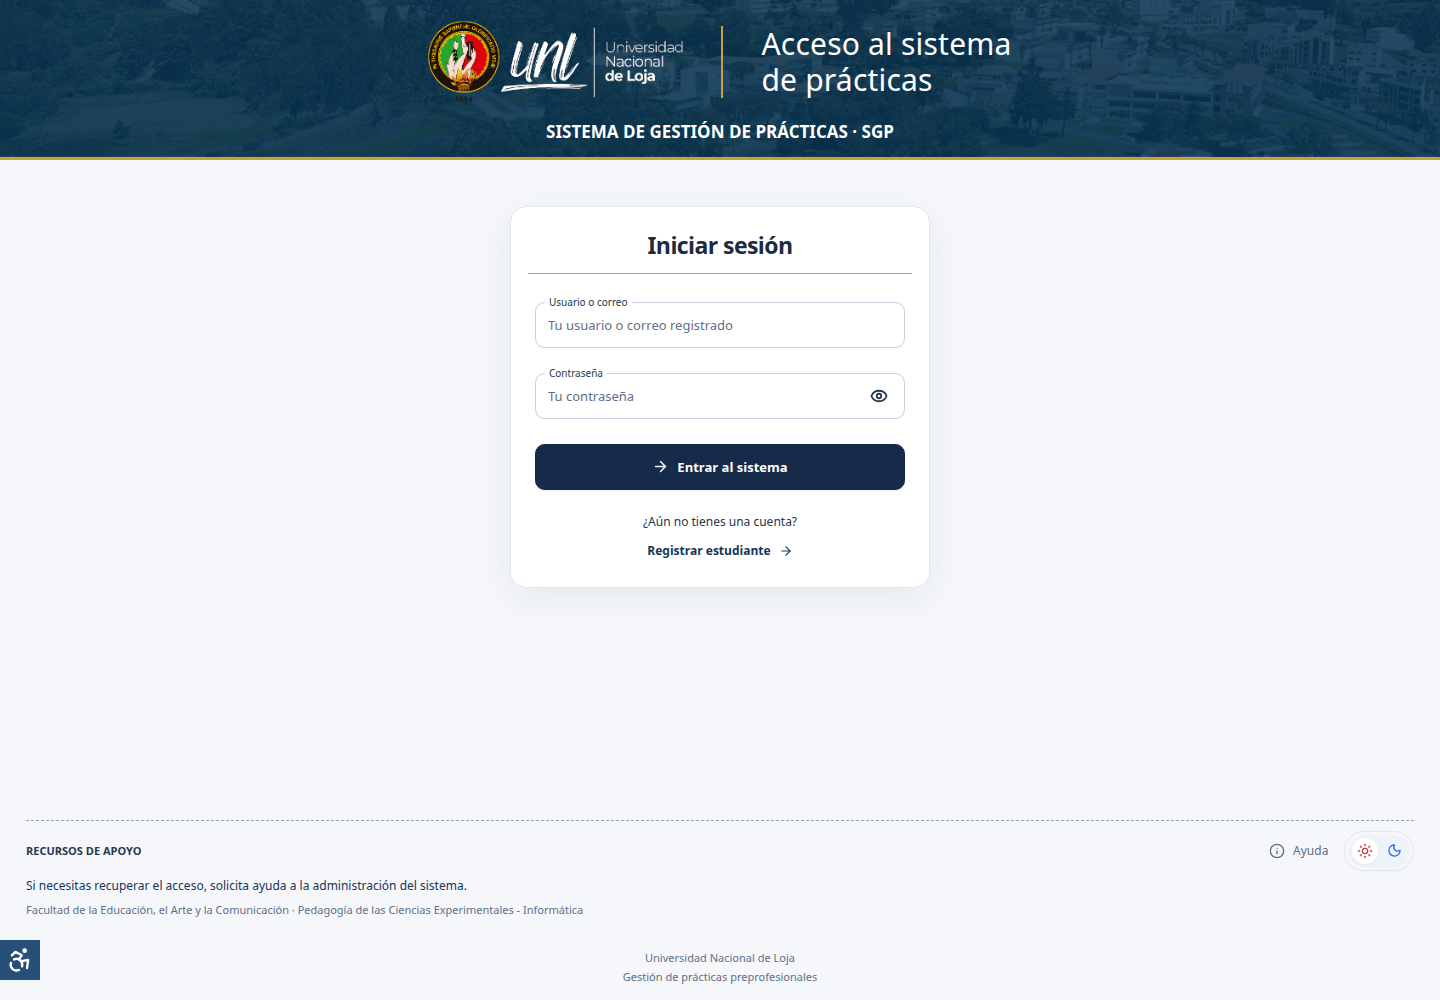
\includegraphics[width=\linewidth,height=0.33\textheight,keepaspectratio]{interfaz-login.png}
\end{center}
\refstepcounter{figure}\label{fig:interfaz-acceso}
{\small\textbf{\figurename~\thefigure.} Usuario o correo, contraseña y entrada al sistema.\par}
\subsection{Asignación administrativa}
\begin{center}
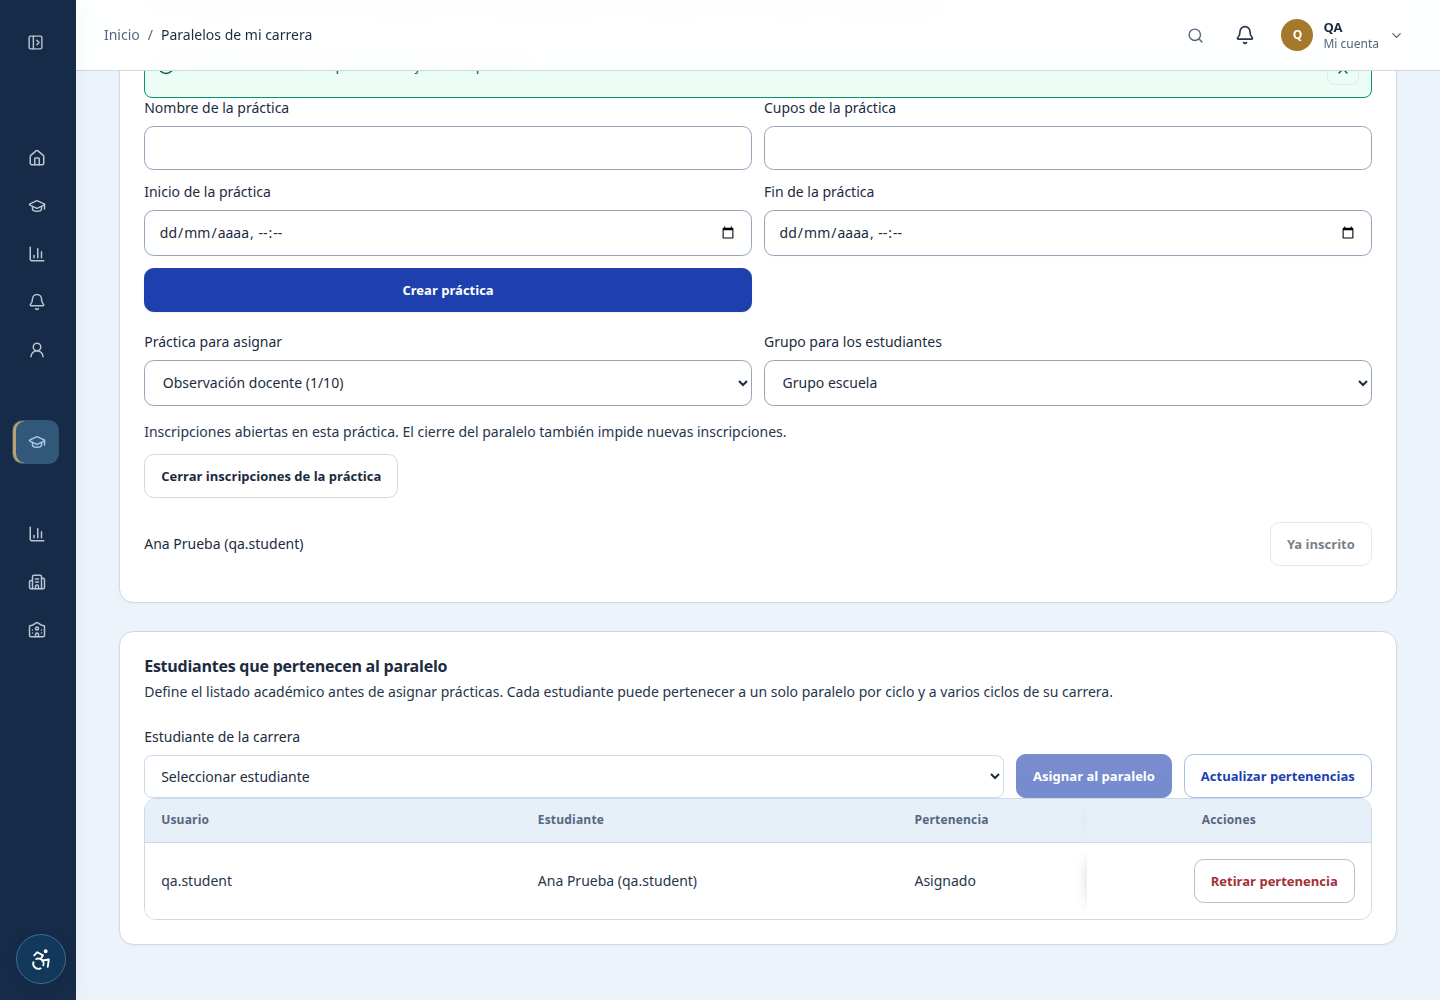
\includegraphics[width=\linewidth,height=0.33\textheight,keepaspectratio]{interfaz-asignacion.png}
\end{center}
\refstepcounter{figure}\label{fig:interfaz-asignacion}
{\small\textbf{\figurename~\thefigure.} El personal autorizado habilita la práctica para el estudiante.\par}
\clearpage
\subsection{Mis prácticas}
\begin{center}
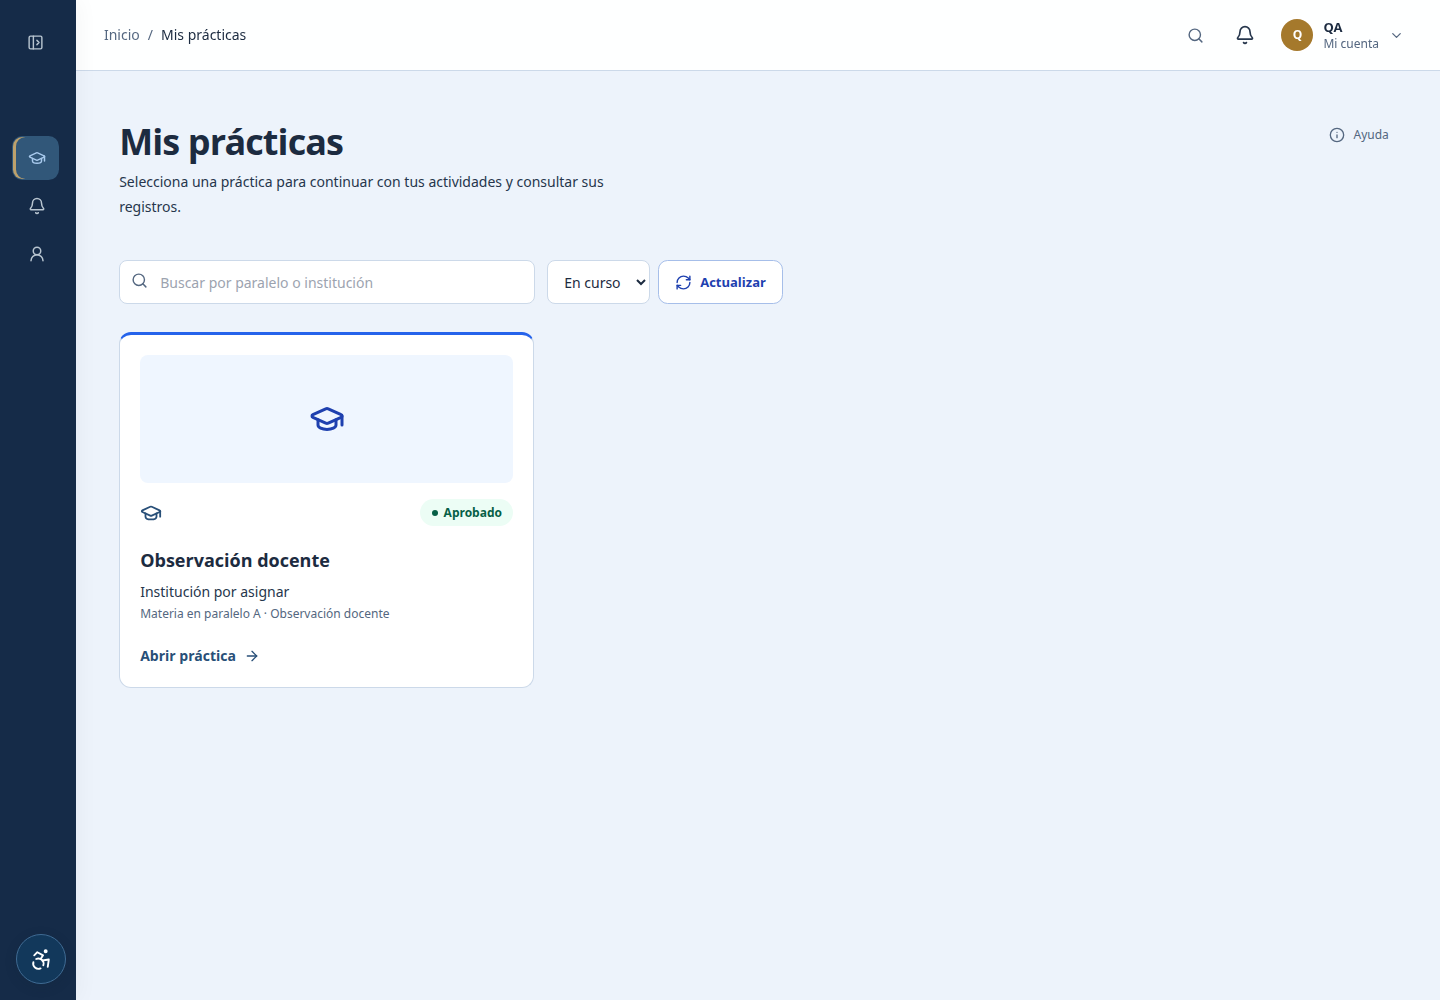
\includegraphics[width=\linewidth,height=0.33\textheight,keepaspectratio]{interfaz-mis-practicas.png}
\end{center}
\refstepcounter{figure}\label{fig:interfaz-mis-practicas}
{\small\textbf{\figurename~\thefigure.} El estudiante consulta sus prácticas y abre el espacio de trabajo.\par}
\subsection{Resumen de la práctica}
\begin{center}
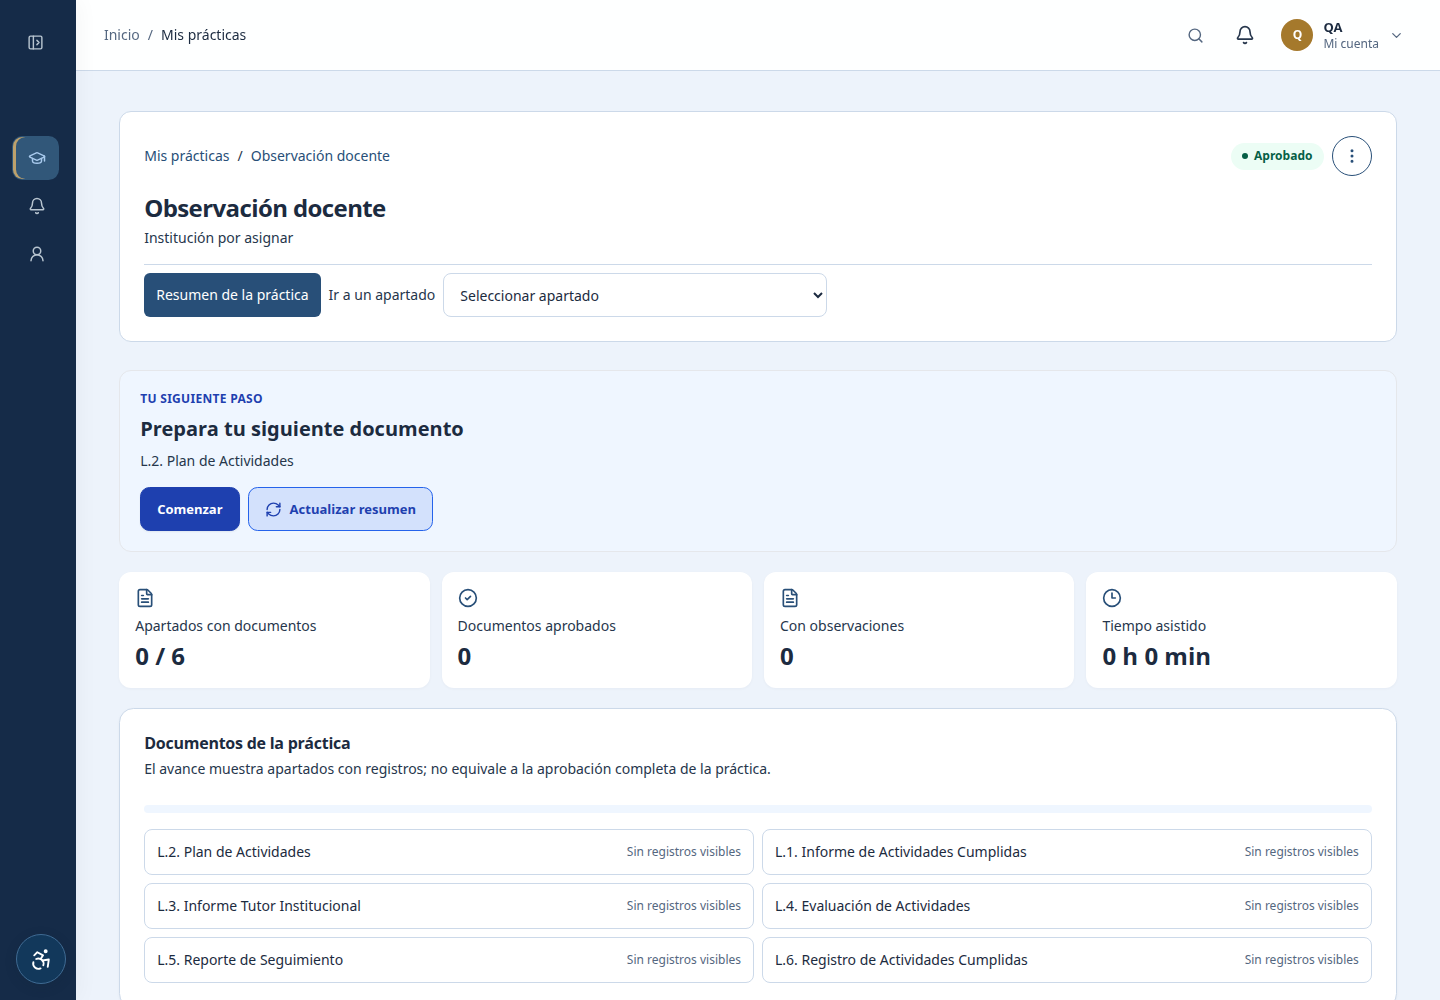
\includegraphics[width=\linewidth,height=0.33\textheight,keepaspectratio]{interfaz-resumen-practica.png}
\end{center}
\refstepcounter{figure}\label{fig:interfaz-resumen}
{\small\textbf{\figurename~\thefigure.} Resumen de la práctica y seguimiento de sus documentos.\par}

\clearpage
\section{Diagramas de casos de uso por rol}
Los siguientes diagramas representan las funciones de los seis roles principales.
Las diferencias entre estas vistas y las reglas actuales de asignación se
explican en la sección 1.2.

\subsection{Administrador}
\begin{center}
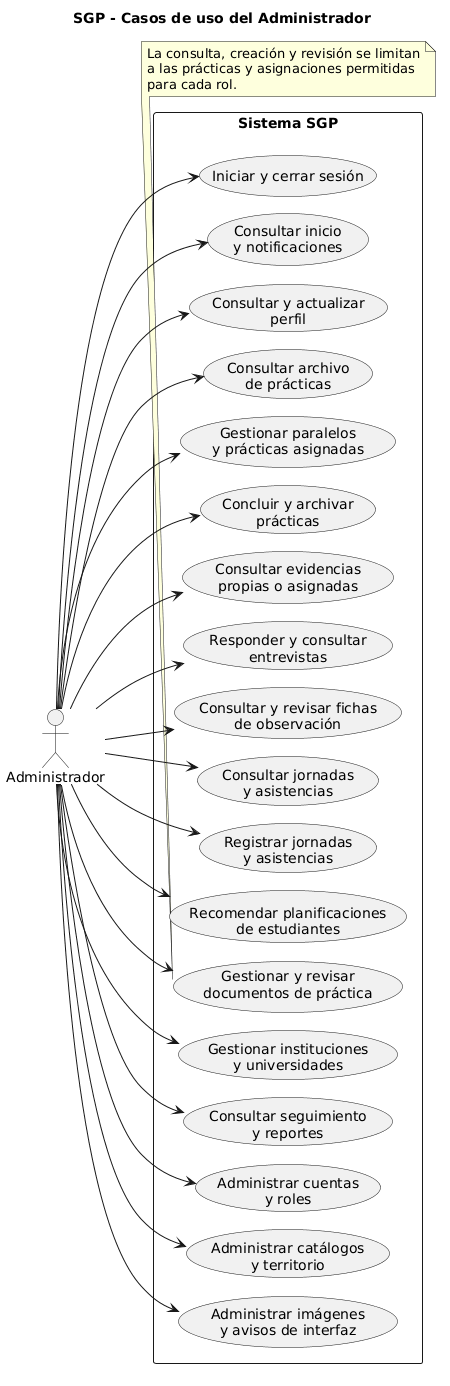
\includegraphics[width=\linewidth,height=0.72\textheight,keepaspectratio]{administrador.png}
\end{center}
\refstepcounter{figure}\label{fig:cu-administrador}
\textbf{\figurename~\thefigure.} Casos de uso: Administrador.
\clearpage
\subsection{Director de prácticas}
\begin{center}
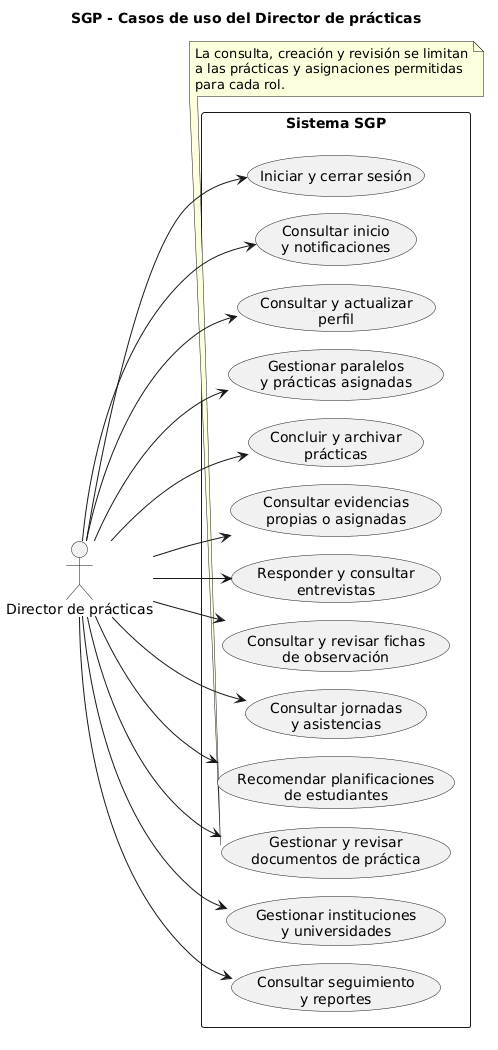
\includegraphics[width=\linewidth,height=0.84\textheight,keepaspectratio]{director-practicas.png}
\end{center}
\refstepcounter{figure}\label{fig:cu-director-practicas}
\textbf{\figurename~\thefigure.} Casos de uso: Director de prácticas.
\clearpage
\subsection{Directora de institución}
\begin{center}
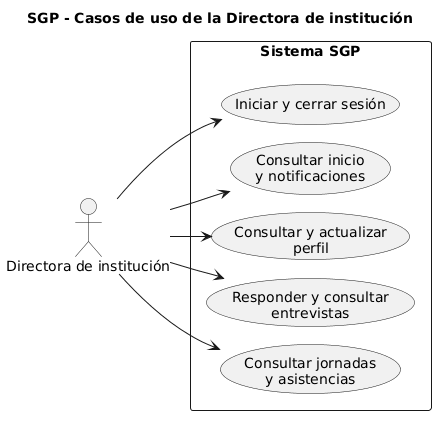
\includegraphics[width=\linewidth,height=0.84\textheight,keepaspectratio]{directora-institucion.png}
\end{center}
\refstepcounter{figure}\label{fig:cu-directora-institucion}
\textbf{\figurename~\thefigure.} Casos de uso: Directora de institución.
\clearpage
\subsection{Estudiante}
\begin{center}
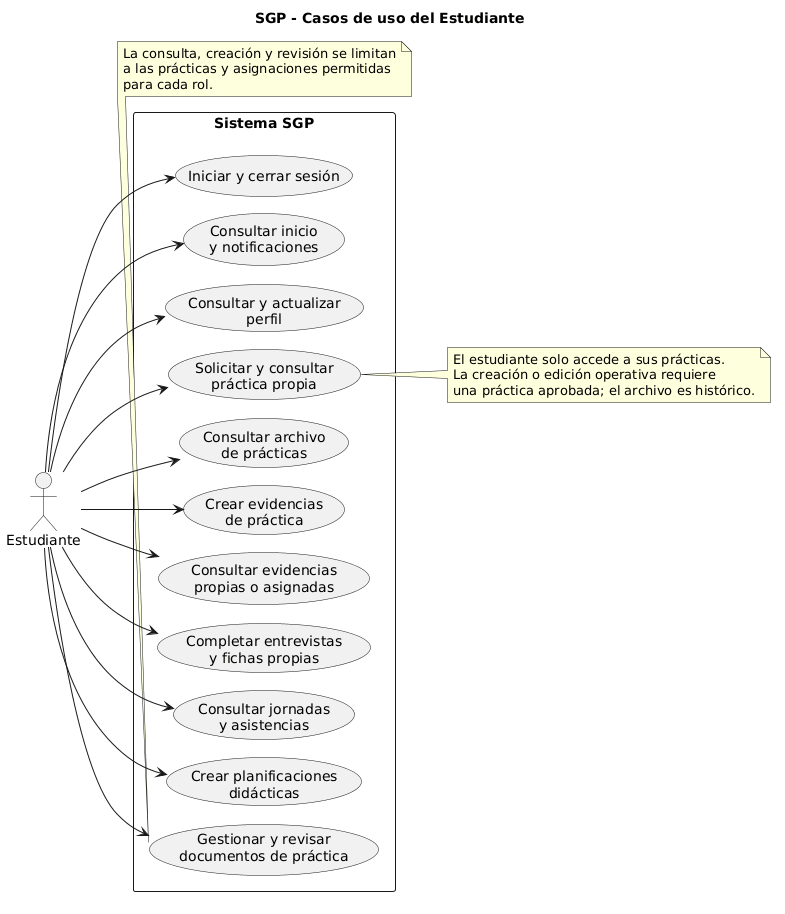
\includegraphics[width=\linewidth,height=0.84\textheight,keepaspectratio]{estudiante.png}
\end{center}
\refstepcounter{figure}\label{fig:cu-estudiante}
\textbf{\figurename~\thefigure.} Casos de uso: Estudiante.
\clearpage
\subsection{Tutor de prácticas}
\begin{center}
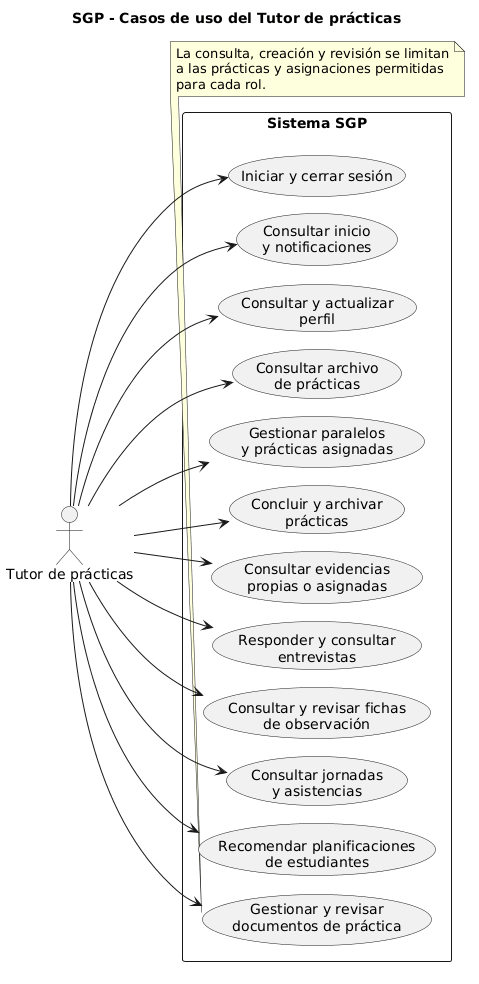
\includegraphics[width=\linewidth,height=0.84\textheight,keepaspectratio]{tutor-practicas.png}
\end{center}
\refstepcounter{figure}\label{fig:cu-tutor-practicas}
\textbf{\figurename~\thefigure.} Casos de uso: Tutor de prácticas.
\clearpage
\subsection{Tutor institucional}
\begin{center}
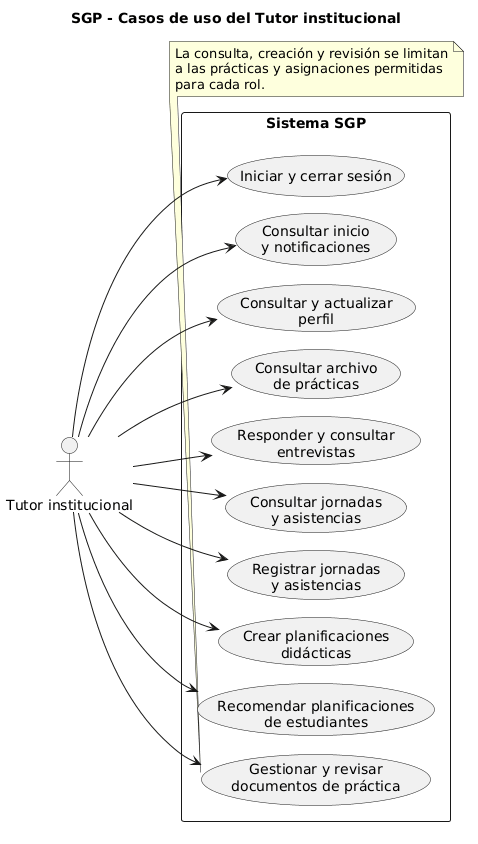
\includegraphics[width=\linewidth,height=0.84\textheight,keepaspectratio]{tutor-institucional.png}
\end{center}
\refstepcounter{figure}\label{fig:cu-tutor-institucional}
\textbf{\figurename~\thefigure.} Casos de uso: Tutor institucional.

\clearpage
\section{Trazabilidad del catálogo}
Las relaciones REQ\_ACT, CU\_ACT y REQ\_CU se presentan como listas de códigos
asociados para evitar matrices muy anchas. Cada lista equivale a las celdas
marcadas de la fila original. Una relación documental no concede permisos.
El signo ``---'' indica que no hay un caso asociado en la matriz fuente.
\subsection{Requisitos, actores y casos relacionados}
En la columna de actores, los números 001--008 equivalen a ACT-001--ACT-008;
en la de casos, 001--026 equivalen a CU-001--CU-026.

{\small
\begin{longtable}{@{}P{2.5cm}P{6.1cm}P{6.2cm}@{}}
\toprule
\textbf{Requisito} & \textbf{Actores (ACT)} & \textbf{Casos (CU)}\\\midrule
\endfirsthead
\toprule
\textbf{Requisito} & \textbf{Actores (ACT)} & \textbf{Casos (CU)}\\\midrule
\endhead
\midrule
\multicolumn{3}{r}{\footnotesize Continúa en la siguiente página.}\\
\endfoot
\bottomrule
\endlastfoot
REQ-F-001 & 001, 002, 003, 004, 005, 006, 007 & 001\\
REQ-F-002 & 001 & 002\\
REQ-F-003 & 001 & 003\\
REQ-F-004 & 001, 007 & 003, 024\\
REQ-F-005 & 001, 007 & 024\\
REQ-F-006 & 002, 007 & 005\\
REQ-F-007 & 002, 007 & 005\\
REQ-F-008 & 002, 003, 005, 006, 007 & 009\\
REQ-F-009 & 002, 003, 005, 006, 007 & 009\\
REQ-F-010 & 002, 003, 005, 006, 007 & 009\\
REQ-F-011 & 002, 003, 005, 006, 007 & 013\\
REQ-F-012 & 002, 003, 005, 006, 007 & 013\\
REQ-F-013 & 002, 003, 005, 006, 007 & 013\\
REQ-F-014 & 002, 003, 005 & 014\\
REQ-F-015 & 002, 005 & 016\\
REQ-F-016 & 002, 005 & 015\\
REQ-F-017 & 002, 003, 005, 006, 007 & 017\\
REQ-F-018 & 002, 003, 004, 005, 006, 007 & 018\\
REQ-F-019 & 002, 003, 005, 006, 007 & 020\\
REQ-F-020 & 002, 003, 004, 005, 006, 007 & 019\\
REQ-F-021 & 002, 003, 004, 005, 006, 007 & 021\\
REQ-F-022 & 002, 003, 004, 005, 006, 007 & 025\\
REQ-F-023 & 002, 003, 004, 005, 006, 007 & 004\\
REQ-F-024 & 002, 003, 005, 006, 007 & 009\\
REQ-F-025 & 002, 003, 004, 005, 006, 007 & 019\\
REQ-F-026 & 002, 003, 004, 005, 006, 007 & 019\\
REQ-F-027 & 002, 003, 005, 006, 007 & 013, 014\\
REQ-F-028 & 002, 003, 005, 006, 007 & 013, 014\\
REQ-F-029 & 002, 003, 004, 005, 006, 007 & 018\\
REQ-F-030 & 002, 003, 005, 006, 007 & 020\\
REQ-F-031 & 002, 003, 005, 006, 007 & 020\\
REQ-F-032 & 002, 003, 005, 006, 007 & 013\\
REQ-F-033 & 002, 003, 004, 005, 006, 007 & 004\\
REQ-F-034 & 002, 003, 004, 005, 006, 007 & 019\\
REQ-F-035 & 002, 003, 004, 005, 006, 007 & 018\\
REQ-F-036 & 002, 003, 004, 005, 006, 007 & 004\\
REQ-F-037 & 002, 005, 006, 007 & 008\\
REQ-F-038 & 005, 007 & 010\\
REQ-F-039 & 002, 003, 005, 006, 007 & 013, 014\\
REQ-F-040 & 002, 003, 005, 006, 007 & 013, 014\\
REQ-F-041 & 002, 005 & 015\\
REQ-F-042 & 002, 005 & 015\\
REQ-F-043 & 002, 005 & 016\\
REQ-F-044 & 002, 003, 004, 005, 006, 007 & 017, 018\\
REQ-F-045 & 002, 003, 005, 006, 007 & 020\\
REQ-F-046 & 002, 003, 004, 005, 006, 007 & 019\\
REQ-F-047 & 002, 003, 004, 005, 006, 007 & 025\\
REQ-F-048 & 002, 003, 004, 005, 006, 007 & 004\\
REQ-F-049 & 005, 006, 007 & 007\\
REQ-F-050 & 006, 007 & 006\\
REQ-F-051 & 002, 006, 007 & 008\\
REQ-F-052 & 002, 003, 005, 006, 007 & 009\\
REQ-F-053 & 006 & 011\\
REQ-F-054 & 003, 005, 006 & 014\\
REQ-F-055 & 002, 003, 004, 005, 006, 007 & 017, 018, 019\\
REQ-F-056 & 006, 007 & 023\\
REQ-F-057 & 002, 003, 005, 006, 007 & 020\\
REQ-F-058 & 002, 003, 004, 005, 006, 007 & 025\\
REQ-F-059 & 007 & 005\\
REQ-F-060 & 007 & 005\\
REQ-F-061 & 007 & 005\\
REQ-F-062 & 007 & 006\\
REQ-F-063 & 007 & 006\\
REQ-F-064 & 007 & 006\\
REQ-F-065 & 002, 006, 007 & 008\\
REQ-F-066 & 002, 003, 005, 006, 007 & 009\\
REQ-F-067 & 007 & 012\\
REQ-F-068 & 002, 003, 005, 006, 007 & 013, 014\\
REQ-F-069 & 007 & 022\\
REQ-F-070 & 006, 007 & 023\\
REQ-F-071 & 001, 007 & 024\\
REQ-F-072 & 002, 003, 005, 006, 007 & 020\\
REQ-F-073 & 002, 003, 004, 005, 006, 007 & 025\\
REQ-F-074 & 001 & 026\\
REQ-NF-001 & 001, 002, 003, 004, 005, 006, 007, 008 & 001\\
REQ-NF-002 & 001, 002, 003, 004, 005, 006, 007, 008 & 001\\
REQ-NF-003 & 001, 002, 003, 004, 005, 006, 007, 008 & 001\\
REQ-NF-004 & 001, 002, 003, 004, 005, 006, 007, 008 & 001, 002, 005, 026\\
REQ-NF-005 & 001, 002, 003, 004, 005, 006, 007, 008 & 002, 004, 013, 017, 020, 024, 025\\
REQ-NF-006 & 001, 002, 003, 004, 005, 006, 007, 008 & 002, 004, 013, 017, 020, 024\\
REQ-NF-007 & 001, 002, 003, 004, 005, 006, 007, 008 & 004, 005, 006, 007, 008, 009, 010, 011, 012, 013, 014, 015, 016, 017, 018, 019, 020, 021, 022, 023, 024, 025\\
REQ-NF-008 & 002, 003, 004, 005, 006, 007, 008 & 008, 009, 010, 011, 012, 013, 014, 015, 016, 017, 018, 019, 020\\
REQ-NF-009 & 002, 003, 005, 006, 007, 008 & 013, 014, 016\\
REQ-NF-010 & 008 & ---\\
REQ-NF-011 & 008 & ---\\
REQ-NF-012 & 008 & ---\\
REQ-NF-013 & 001, 008 & 026\\
\end{longtable}
}
\subsection{Casos de uso y actores participantes}

{\small
\begin{longtable}{@{}P{2.2cm}P{12.9cm}@{}}
\toprule
\textbf{Caso} & \textbf{Actores relacionados}\\\midrule
\endfirsthead
\toprule
\textbf{Caso} & \textbf{Actores relacionados}\\\midrule
\endhead
\midrule
\multicolumn{2}{r}{\footnotesize Continúa en la siguiente página.}\\
\endfoot
\bottomrule
\endlastfoot
CU-001 & ACT-001, ACT-002, ACT-003, ACT-004, ACT-005, ACT-006, ACT-007\\
CU-002 & ACT-001\\
CU-003 & ACT-001\\
CU-004 & ACT-002, ACT-003, ACT-004, ACT-005, ACT-006, ACT-007\\
CU-005 & ACT-007\\
CU-006 & ACT-007\\
CU-007 & ACT-005, ACT-006, ACT-007\\
CU-008 & ACT-002, ACT-006, ACT-007\\
CU-009 & ACT-002, ACT-003, ACT-005, ACT-006, ACT-007\\
CU-010 & ACT-005, ACT-007\\
CU-011 & ACT-006\\
CU-012 & ACT-007\\
CU-013 & ACT-002, ACT-003, ACT-005, ACT-006, ACT-007\\
CU-014 & ACT-003, ACT-005\\
CU-015 & ACT-002, ACT-005\\
CU-016 & ACT-002, ACT-005\\
CU-017 & ACT-002, ACT-003, ACT-005, ACT-006, ACT-007\\
CU-018 & ACT-002, ACT-003, ACT-004, ACT-005, ACT-006, ACT-007\\
CU-019 & ACT-002, ACT-003, ACT-004, ACT-005, ACT-006, ACT-007\\
CU-020 & ACT-002, ACT-003, ACT-005, ACT-006, ACT-007\\
CU-021 & ACT-002, ACT-003, ACT-004, ACT-005, ACT-006, ACT-007\\
CU-022 & ACT-007\\
CU-023 & ACT-006, ACT-007\\
CU-024 & ACT-001, ACT-007\\
CU-025 & ACT-002, ACT-003, ACT-004, ACT-005, ACT-006, ACT-007\\
CU-026 & ACT-001\\
\end{longtable}
}
\clearpage
\section{Secuencias principales del sistema}
Cuatro modelos de síntesis muestran el recorrido correcto y sus alternativas al pie.
Las llamadas internas se agrupan; fuentes editables: \ruta{docs/bitacora/diagramas/}.

\subsection{Inicio de sesión}
\begin{center}
\setlength{\unitlength}{0.8mm}
\begin{picture}(180,83.0)(0,-76.0)
\small\color{azul}
\put(12,0){\makebox(0,0){\shortstack{Usuario}}}
\multiput(12,-6)(0,-3){23}{\line(0,-1){1.5}}
\put(54,0){\makebox(0,0){\shortstack{Pantalla}}}
\multiput(54,-6)(0,-3){23}{\line(0,-1){1.5}}
\put(106,0){\makebox(0,0){\shortstack{Autenticación}}}
\multiput(106,-6)(0,-3){23}{\line(0,-1){1.5}}
\put(158,0){\makebox(0,0){\shortstack{Base de\\datos}}}
\multiput(158,-6)(0,-3){23}{\line(0,-1){1.5}}
\color{black}
\msg{12}{42}{16.0}{1}{1. Introducir usuario/correo y contraseña}
\msg{54}{52}{22.0}{1}{2. POST /api/auth/login}
\msg{106}{52}{28.0}{1}{3. Buscar cuenta no eliminada}
\ret{158}{52}{34.0}{-1}{4. Cuenta, hash y roles}
\local{106}{40.0}{5. Verificar estado y BCrypt}
\ret{106}{52}{46.0}{-1}{6. Emitir JWT y estado de contraseña}
\local{54}{52.0}{7. Guardar autenticación}
\msg{54}{52}{58.0}{1}{8. GET /api/account/me con Bearer}
\local{106}{64.0}{9. Validar JWT, cuenta y roles}
\ret{106}{52}{70.0}{-1}{10. Perfil autorizado}
\ret{54}{42}{76.0}{-1}{11. Cambio de contraseña o panel autorizado}
\end{picture}
\end{center}
\refstepcounter{figure}\label{fig:seq-login-resumen}
\textbf{\figurename~\thefigure.} Inicio de sesión.

{\footnotesize La columna Autenticación agrupa la API, Spring Security y el servicio JWT. Si las credenciales o la cuenta se rechazan, se muestra el error; si falla la consulta del perfil, se elimina la autenticación local. BCrypt verifica un hash y los JWT se firman, sin cifrar su contenido.\par}

\subsection{Asignación administrativa de una práctica}
\begin{center}
\setlength{\unitlength}{0.8mm}
\begin{picture}(180,77.0)(0,-70.0)
\small\color{azul}
\put(12,0){\makebox(0,0){\shortstack{Personal\\autorizado}}}
\multiput(12,-6)(0,-3){21}{\line(0,-1){1.5}}
\put(54,0){\makebox(0,0){\shortstack{Pantalla}}}
\multiput(54,-6)(0,-3){21}{\line(0,-1){1.5}}
\put(106,0){\makebox(0,0){\shortstack{Servicio SGP}}}
\multiput(106,-6)(0,-3){21}{\line(0,-1){1.5}}
\put(158,0){\makebox(0,0){\shortstack{Base de\\datos}}}
\multiput(158,-6)(0,-3){21}{\line(0,-1){1.5}}
\color{black}
\msg{12}{42}{16.0}{1}{1. Seleccionar práctica, estudiante y grupo}
\msg{54}{52}{22.0}{1}{2. Solicitar inscripción administrativa}
\msg{106}{52}{28.0}{1}{3. Cargar práctica, paralelo y estudiante}
\ret{158}{52}{34.0}{-1}{4. Datos y pertenencia académica}
\local{106}{40.0}{5. Validar ámbito, cupos, apertura y tutores}
\msg{106}{52}{46.0}{1}{6. Guardar inscripción APPROVED e historial}
\ret{158}{52}{52.0}{-1}{7. Inscripción persistida}
\local{106}{58.0}{8. Generar notificación al estudiante}
\ret{106}{52}{64.0}{-1}{9. Práctica habilitada}
\ret{54}{42}{70.0}{-1}{10. Mostrar asignación confirmada}
\end{picture}
\end{center}
\refstepcounter{figure}\label{fig:seq-asignacion-practica}
\textbf{\figurename~\thefigure.} Asignación administrativa de una práctica.

{\footnotesize Intervienen administración, dirección o tutor de prácticas dentro de su ámbito. Si no se cumplen pertenencia, cupos, apertura o tutores habilitados, se rechaza la asignación; el estudiante no se autoinscribe.\par}

\clearpage
\subsection{Envío y revisión de un plan de actividades}
\begin{center}
\setlength{\unitlength}{0.8mm}
\begin{picture}(180,77.0)(0,-70.0)
\small\color{azul}
\put(12,0){\makebox(0,0){\shortstack{Estudiante /\\tutor}}}
\multiput(12,-6)(0,-3){21}{\line(0,-1){1.5}}
\put(54,0){\makebox(0,0){\shortstack{Pantalla}}}
\multiput(54,-6)(0,-3){21}{\line(0,-1){1.5}}
\put(106,0){\makebox(0,0){\shortstack{Servicio SGP}}}
\multiput(106,-6)(0,-3){21}{\line(0,-1){1.5}}
\put(158,0){\makebox(0,0){\shortstack{Base de\\datos}}}
\multiput(158,-6)(0,-3){21}{\line(0,-1){1.5}}
\color{black}
\msg{12}{42}{16.0}{1}{1. Estudiante: enviar plan guardado}
\msg{54}{52}{22.0}{1}{2. Enviar plan para revisión}
\local{106}{28.0}{3. Comprobar propiedad, edición y transición}
\msg{106}{52}{34.0}{1}{4. Guardar SUBMITTED y ciclo de revisión}
\ret{106}{52}{40.0}{-1}{5. Confirmar envío y notificar revisión}
\msg{12}{42}{46.0}{1}{6. Tutor autorizado: revisar y comentar}
\msg{54}{52}{52.0}{1}{7. Enviar decisión o retroalimentación}
\local{106}{58.0}{8. Validar revisor, práctica y estado}
\msg{106}{52}{64.0}{1}{9. Guardar revisión, comentarios e historial}
\ret{106}{52}{70.0}{-1}{10. Devolver estado y notificar al estudiante}
\end{picture}
\end{center}
\refstepcounter{figure}\label{fig:seq-revision-documento}
\textbf{\figurename~\thefigure.} Envío y revisión de un plan de actividades.

{\footnotesize La primera línea de vida agrupa dos actores que actúan en momentos distintos. El plan de actividades ejemplifica CU-013 y CU-014; los demás documentos pueden tener etapas propias y no se presumen idénticos.\par}

\subsection{Conclusión y archivo de una práctica}
\begin{center}
\setlength{\unitlength}{0.8mm}
\begin{picture}(180,83.0)(0,-76.0)
\small\color{azul}
\put(12,0){\makebox(0,0){\shortstack{Dirección /\\administración}}}
\multiput(12,-6)(0,-3){23}{\line(0,-1){1.5}}
\put(54,0){\makebox(0,0){\shortstack{Pantalla}}}
\multiput(54,-6)(0,-3){23}{\line(0,-1){1.5}}
\put(106,0){\makebox(0,0){\shortstack{Servicio SGP}}}
\multiput(106,-6)(0,-3){23}{\line(0,-1){1.5}}
\put(158,0){\makebox(0,0){\shortstack{Base de\\datos}}}
\multiput(158,-6)(0,-3){23}{\line(0,-1){1.5}}
\color{black}
\msg{12}{42}{16.0}{1}{1. Dirección: consultar resumen de cierre}
\msg{54}{52}{22.0}{1}{2. Solicitar resumen y advertencias}
\ret{106}{52}{28.0}{-1}{3. Documentos, horas y pendientes}
\msg{12}{42}{34.0}{1}{4. Dirección: confirmar conclusión manual}
\msg{54}{52}{40.0}{1}{5. Solicitar conclusión}
\msg{106}{52}{46.0}{1}{6. Guardar COMPLETED y auditoría}
\msg{12}{42}{52.0}{1}{7. Administración: archivar práctica}
\msg{54}{52}{58.0}{1}{8. Solicitar archivo}
\local{106}{64.0}{9. Validar administrador y estado COMPLETED}
\msg{106}{52}{70.0}{1}{10. Guardar archivo, fecha y auditoría}
\ret{106}{52}{76.0}{-1}{11. Confirmar consulta histórica}
\end{picture}
\end{center}
\refstepcounter{figure}\label{fig:seq-cierre-archivo}
\textbf{\figurename~\thefigure.} Conclusión y archivo de una práctica.

{\footnotesize La dirección concluye y la administración archiva, en operaciones distintas (CU-011 y CU-012). Los pendientes se muestran como advertencias: ni el vencimiento del período ni el cierre de inscripciones concluyen automáticamente una práctica.\par}


\clearpage
\section{Algoritmos relevantes de la implementación}
Los siguientes algoritmos resuelven reglas específicas del sistema. Presento
los fragmentos relevantes de la implementación y un ejemplo de su funcionamiento.
La numeración del margen identifica las líneas del archivo de origen.

\subsection{Transiciones de revisión documental}
La máquina de estados define qué cambios admite cada estado. El método
\texttt{transition} consulta esa tabla y rechaza una transición no prevista.
Se muestran dos fragmentos separados del mismo archivo.

\begin{lstlisting}[style=sgpjava,firstnumber=27]
private static final Map<String, Set<String>> ALLOWED_TRANSITIONS = Map.of(
        DRAFT, Set.of(SUBMITTED),
        SUBMITTED, Set.of(DRAFT, SUBMITTED, NEEDS_CORRECTION, APPROVED),
        NEEDS_CORRECTION, Set.of(SUBMITTED),
        APPROVED, Set.of());
\end{lstlisting}
\begin{lstlisting}[style=sgpjava,firstnumber=62]
if (!ALLOWED_TRANSITIONS.getOrDefault(current, Set.of()).contains(next)) {
    throw new BadRequestException(
            "Transicion de estado no permitida para "
                    + documentName
                    + ": "
                    + current
                    + " -> "
                    + next);
}

return nextStatus;
\end{lstlisting}

\textbf{Ejemplo.} Un borrador puede enviarse a revisión; un documento aprobado no
admite nuevas transiciones mediante esta tabla. Las comprobaciones de propiedad,
rol y práctica operativa se realizan en los servicios que la utilizan.

{\small\textbf{Origen:} \texttt{ReviewWorkflowStateMachine.java}, líneas 27--31 y 62--72.\par}

\subsection{Detección de solapamiento de asistencias}
Dos franjas se solapan si cada una comienza antes de que termine la otra.
El método comprueba primero que las cuatro horas estén disponibles.

\begin{lstlisting}[style=sgpjava,firstnumber=721]
private boolean attendanceTimesOverlap(PracticeAttendance existing, PracticeAttendance attendance) {
    return existing.getStartTime() != null && existing.getEndTime() != null
            && attendance.getStartTime() != null && attendance.getEndTime() != null
            && existing.getStartTime().isBefore(attendance.getEndTime())
            && attendance.getStartTime().isBefore(existing.getEndTime());
}
\end{lstlisting}

\textbf{Ejemplo.} 08:00--09:00 y 08:30--09:30 se solapan; 08:00--09:00 y
09:00--10:00 no. El método que lo invoca filtra por fecha y excluye el propio
registro al editar; también comprueba duplicados del período.

{\small\textbf{Origen:} \texttt{PracticeScheduleService.java}, líneas 721--726;\newline
contexto de uso: \texttt{validateDuplicateAttendance}, líneas 699--719.\par}

\clearpage
\subsection{Control de versiones de borradores}
Al guardar, el servicio bloquea al propietario y recupera su borrador. Si la
revisión recibida difiere de la almacenada, devuelve un conflicto; si coincide,
guarda el contenido e incrementa la revisión. El bloqueo serializa las escrituras
incluso cuando el borrador aún no existe.

\begin{lstlisting}[style=sgpjava,firstnumber=48]
// Serialize writes for this owner, including first creation and clearing a draft.
var owner = accounts.lockDraftOwner(username).orElseThrow(() -> new ResponseStatusException(HttpStatus.FORBIDDEN));
var draft = drafts.findByOwner_IdAndScope(owner.getId(), scope).orElseGet(() -> {
    var created = new WorkspaceDraft(); created.setOwner(owner); created.setScope(scope); return created;
});
if (revision != draft.getRevision()) throw new ResponseStatusException(HttpStatus.CONFLICT,
        "Este borrador cambió en otra pestaña o dispositivo. Recupera la versión del servidor antes de continuar.");
draft.setContent(content); draft.setRevision(revision + 1); draft.setSavedAt(LocalDateTime.now());
return snapshot(drafts.saveAndFlush(draft));
\end{lstlisting}

\textbf{Ejemplo.} Dos pestañas parten de la revisión 4. La primera guarda la
revisión 5; la segunda, al enviar todavía la 4, recibe HTTP 409 y debe recuperar
la versión del servidor antes de continuar. La autorización y la validación del
objeto JSON se efectúan antes del fragmento.

{\small\textbf{Origen:} \texttt{WorkspaceDraftService.java}, método \texttt{save}, líneas 48--56.\par}

\nota{Los tres archivos pertenecen a
\ruta{BackEnd/src/main/java/com/sgp/systemsgp/service/}.
Los fragmentos forman parte de los servicios de revisión documental, jornadas
y borradores del proyecto.}

\section{Resultados y trabajo pendiente}
\subsection{Resultados del proyecto}
El trabajo documentado comprende ocho actores, 87 requisitos,
26 casos de uso, seis diagramas por rol, las tres relaciones de trazabilidad,
cuatro capturas, cuatro secuencias resumidas y tres algoritmos comentados. Los informes y artefactos permiten consultar el detalle de cada etapa.

\subsection{Pendientes identificados}
\begin{itemize}
\item Conciliar requisitos, casos y relaciones sobre inscripciones con la política
de asignación administrativa del 9 de noviembre.
\item Sincronizar el diagrama general de casos de uso con los 26 casos del catálogo.
\item Ampliar las secuencias solo cuando una nueva regla lo requiera; mantener
los detalles en las fuentes editables para conservar una lectura breve.
\end{itemize}

\clearpage
\section{Referencias documentales}
Todas las rutas se expresan desde la raíz \texttt{SGPv1}. Los informes de
verificación se encuentran en \ruta{docs/testing/informes/}. Las imágenes del proyecto se encuentran
en \ruta{docs/bitacora/imagenes/}; su procedencia se detalla en
\ruta{docs/bitacora/README.md}.
\begin{enumerate}
\item \ruta{README.md} y \ruta{docs/README.md}: componentes e índice documental.
\item \ruta{docs/requisitos/especificacion.md}: catálogo de requisitos y relaciones.
\item \ruta{docs/requisitos/artefactos/diagrama-casos-de-uso.puml}: modelo general anterior.
\item \ruta{docs/requisitos/secuencia-login.md}: explicación y fuentes del login.
\item \ruta{docs/requisitos/artefactos/diagrama-secuencia-login.puml}: secuencia original.
\item \ruta{docs/producto/permisos-practicas.md}: permisos y ámbitos.
\item \ruta{docs/testing/README.md}: alcance de verificaciones y reproducción.
\item \ruta{docs/testing/informes/}: evidencia fechada de evolución del proyecto.
\end{enumerate}
\end{document}
